\documentclass[border=0.2cm]{standalone}
 
% More defined colors
\usepackage[dvipsnames]{xcolor}

 
% Required package
\usepackage{tikz}
\usetikzlibrary{positioning}

\tikzset{arrow/.style = {thick,->,>=stealth,}}


%  colors
\definecolor{M1}{rgb}{1.0, 0.88, 0.21}
\definecolor{M2}{rgb}{0.96, 0.76, 0.76}
\definecolor{M3}{rgb}{0.52, 0.52, 0.51}
\definecolor{M4}{rgb}{0.57, 0.36, 0.51}
\definecolor{M5}{rgb}{0.64, 0.76, 0.68}

\definecolor{B1}{rgb}{0.53, 0.66, 0.42}
\definecolor{B2}{rgb}{0.63, 0.79, 0.95}
\definecolor{B3}{rgb}{1.0, 0.6, 0.4}

\definecolor{layer}{rgb}{0.23, 0.27, 0.29}
\definecolor{add}{rgb}{0.91, 0.84, 0.42}
\begin{document}
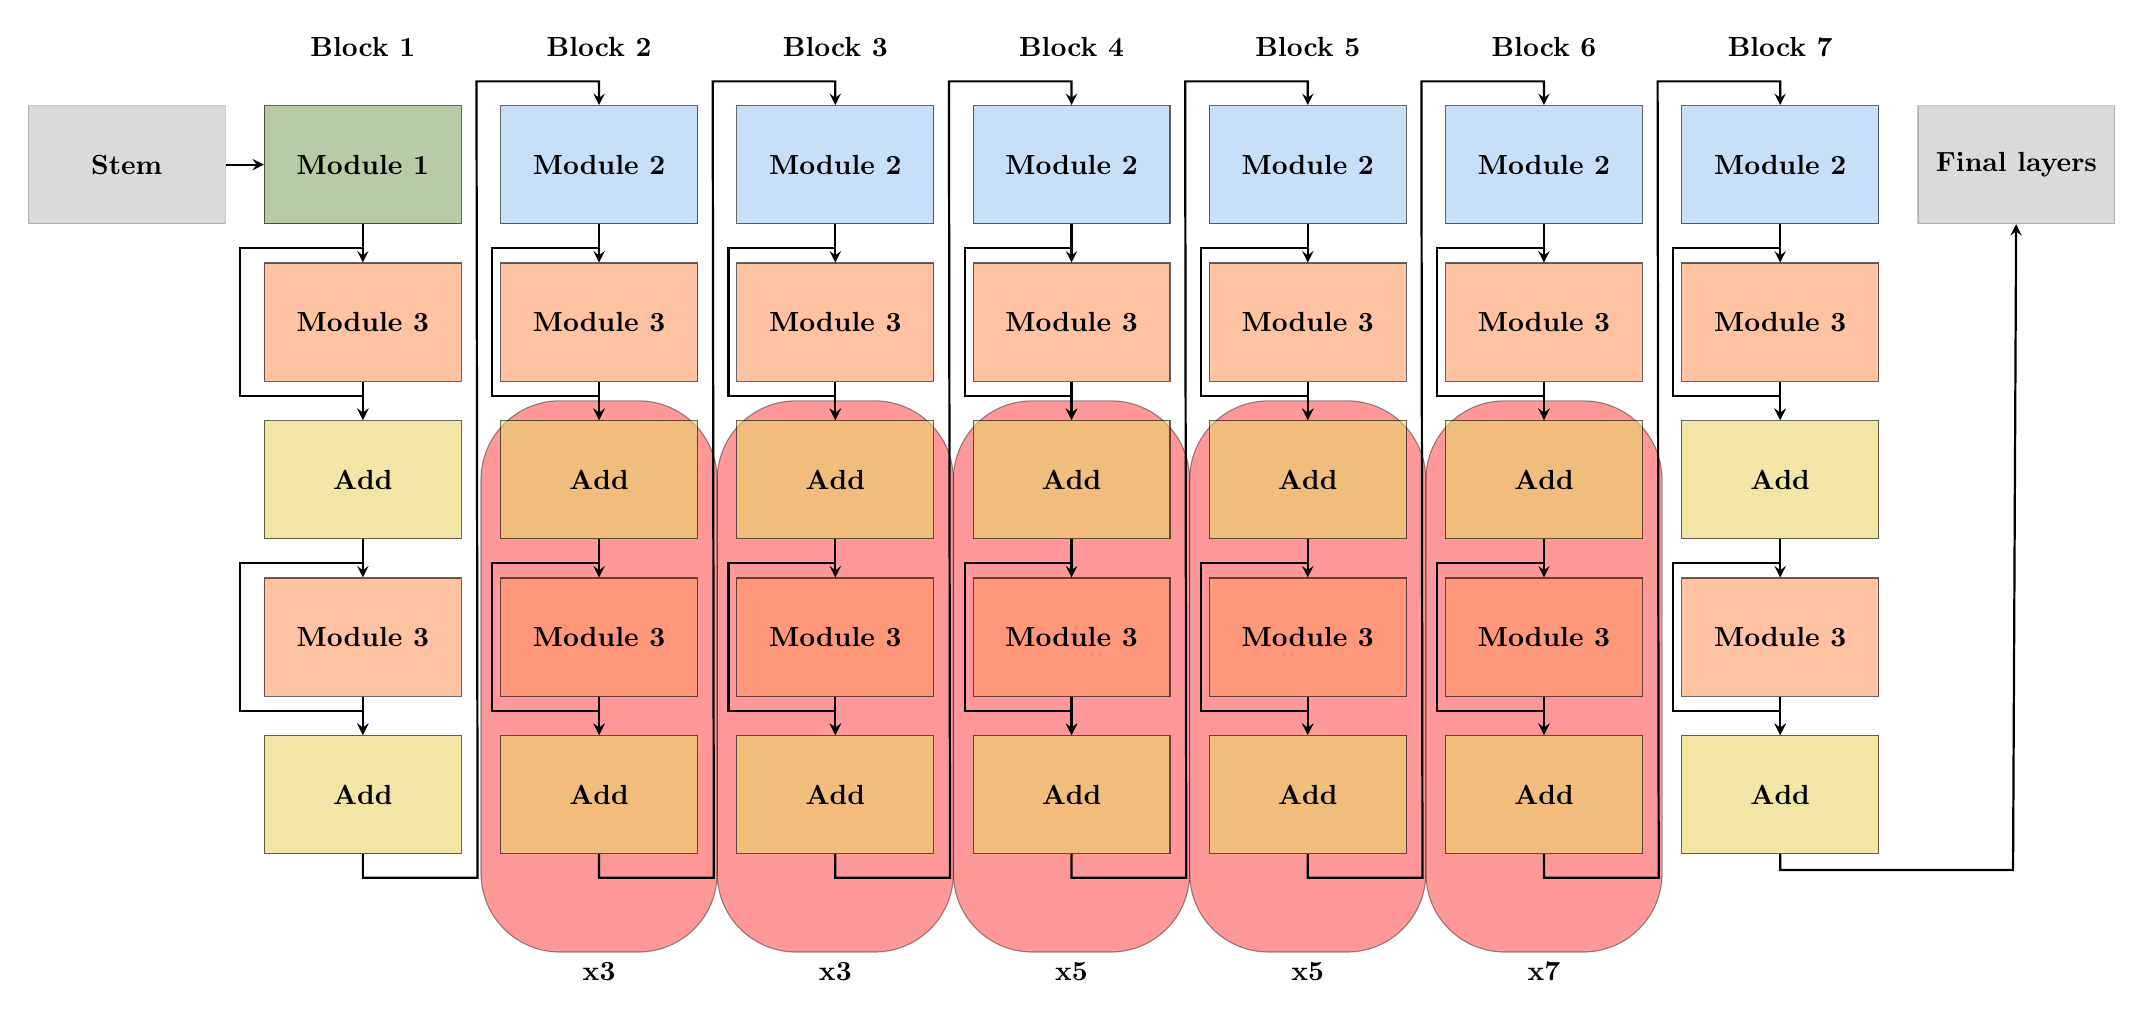
\begin{tikzpicture}

% block name 
\node (text) at (3,1.5) {\textbf{Block 1}};
\node (text) at (6,1.5) {\textbf{Block 2}};
\node (text) at (9,1.5) {\textbf{Block 3}};
\node (text) at (12,1.5) {\textbf{Block 4}};
\node (text) at (15,1.5) {\textbf{Block 5}};
\node (text) at (18,1.5) {\textbf{Block 6}};
\node (text) at (21,1.5) {\textbf{Block 7}};



% Red 
\node [draw,
    fill= red,
    minimum width=3cm,
    minimum height=7cm,
    opacity=0.4,
    rounded corners=1cm,
]  (C1) at (6,-6.5) {} ;
\node (text) at (6,-10.25) {\textbf{x3}};

\node [draw,
    fill= red,
    minimum width=3cm,
    minimum height=7cm,
    opacity=0.4,
    rounded corners=1cm,
]  (C2) at (9,-6.5) {} ;
\node (text) at (9,-10.25) {\textbf{x3}};

\node [draw,
    fill= red,
    minimum width=3cm,
    minimum height=7cm,
    opacity=0.4,
    rounded corners=1cm,
]  (C3) at (12,-6.5) {} ;
\node (text) at (12,-10.25) {\textbf{x5}};

\node [draw,
    fill= red,
    minimum width=3cm,
    minimum height=7cm,
    opacity=0.4,
    rounded corners=1cm,
]  (C3) at (15,-6.5) {} ;
\node (text) at (15,-10.25) {\textbf{x5}};

\node [draw,
    fill= red,
    minimum width=3cm,
    minimum height=7cm,
    opacity=0.4,
    rounded corners=1cm,
]  (C3) at (18,-6.5) {} ;
\node (text) at (18,-10.25) {\textbf{x7}};

% First
\node [draw,
    fill= layer,
    minimum width=2.5cm,
    minimum height=1.5cm,
    opacity=0.2,
]  (F) at (0,0) {} ;
\node (text) at (0,0) {\textbf{Stem}};

% Block1
\node [draw,
    fill= B1,
    minimum width=2.5cm,
    minimum height=1.5cm,
    opacity=0.6,
]  (S1) at (3,0) {} ;
\node (text) at (3,0) {\textbf{Module 1}};


\node [draw,
    fill= B3,
    minimum width=2.5cm,
    minimum height=1.5cm,
    opacity=0.6,
]  (S2) at (3,-2) {} ;
\node (text) at (3,-2) {\textbf{Module 3}};

\node [draw,
    fill= add,
    minimum width=2.5cm,
    minimum height=1.5cm,
    opacity=0.6,
]  (S3) at (3,-4) {} ;
\node (text) at (3,-4) {\textbf{Add}};

 \node [draw,
    fill= B3,
    minimum width=2.5cm,
    minimum height=1.5cm,
    opacity=0.6,
]  (S4) at (3,-6) {} ;
\node (text) at (3,-6) {\textbf{Module 3}};


\node [draw,
    fill= add,
    minimum width=2.5cm,
    minimum height=1.5cm,
    opacity=0.6,
]  (S5) at (3,-8) {} ;
\node (text) at (3,-8) {\textbf{Add}};


%arrows
\draw [arrow] (F) -- (S1);
\draw [arrow] (S1) -- (S2);
\draw [arrow] (S2) -- (S3);
\draw [arrow] (S3) -- (S4);
\draw [arrow] (S4) -- (S5);

\draw [arrow] (S1) |-([shift={(-3mm,-3mm)}]S1.south west)-- ([shift={(-3mm,3mm)}]S3.north west)-|(S3);
\draw [arrow] (S3) |-([shift={(-3mm,-3mm)}]S3.south west)-- ([shift={(-3mm,3mm)}]S5.north west)-|(S5);

%%%%%%%%%%%%%%%%%%%%%%%%%%%%%%%%
% Block 2
\node [draw,
    fill= B2,
    minimum width=2.5cm,
    minimum height=1.5cm,
    opacity=0.6,
]  (T1) at (6,0) {} ;
\node (text) at (6,0) {\textbf{Module 2}};
\draw [arrow] (S5) |-([shift={(2mm,-3mm)}]S5.south east)-- ([shift={(-3mm,3mm)}]T1.north west)-|(T1);


\node [draw,
    fill= B3,
    minimum width=2.5cm,
    minimum height=1.5cm,
    opacity=0.6,
]  (T2) at (6,-2) {} ;
\node (text) at (6,-2) {\textbf{Module 3}};

\node [draw,
    fill= add,
    minimum width=2.5cm,
    minimum height=1.5cm,
    opacity=0.6,
]  (T3) at (6,-4) {} ;
\node (text) at (6,-4) {\textbf{Add}};

 \node [draw,
    fill= B3,
    minimum width=2.5cm,
    minimum height=1.5cm,
    opacity=0.6,
]  (T4) at (6,-6) {} ;
\node (text) at (6,-6) {\textbf{Module 3}};


\node [draw,
    fill= add,
    minimum width=2.5cm,
    minimum height=1.5cm,
    opacity=0.6,
]  (T5) at (6,-8) {} ;
\node (text) at (6,-8) {\textbf{Add}};


%arrows
\draw [arrow] (T1) -- (T2);
\draw [arrow] (T2) -- (T3);
\draw [arrow] (T3) -- (T4);
\draw [arrow] (T4) -- (T5);

\draw [arrow] (T1) |-([shift={(-1mm,-3mm)}]T1.south west)-- ([shift={(-1mm,3mm)}]T3.north west)-|(T3);
\draw [arrow] (T3) |-([shift={(-1mm,-3mm)}]T3.south west)-- ([shift={(-1mm,3mm)}]T5.north west)-|(T5);

%%%%%%%%%%%%%%%%%%%%%%%%%%%%%%%%
% Block 3
\node [draw,
    fill= B2,
    minimum width=2.5cm,
    minimum height=1.5cm,
    opacity=0.6,
]  (F1) at (9,0) {} ;
\node (text) at (9,0) {\textbf{Module 2}};

\draw [arrow] (T5) |-([shift={(2mm,-3mm)}]T5.south east)-- ([shift={(-3mm,3mm)}]F1.north west)-|(F1);

\node [draw,
    fill= B3,
    minimum width=2.5cm,
    minimum height=1.5cm,
    opacity=0.6,
]  (F2) at (9,-2) {} ;
\node (text) at (9,-2) {\textbf{Module 3}};

\node [draw,
    fill= add,
    minimum width=2.5cm,
    minimum height=1.5cm,
    opacity=0.6,
]  (F3) at (9,-4) {} ;
\node (text) at (9,-4) {\textbf{Add}};

 \node [draw,
    fill= B3,
    minimum width=2.5cm,
    minimum height=1.5cm,
    opacity=0.6,
]  (F4) at (9,-6) {} ;
\node (text) at (9,-6) {\textbf{Module 3}};


\node [draw,
    fill= add,
    minimum width=2.5cm,
    minimum height=1.5cm,
    opacity=0.6,
]  (F5) at (9,-8) {} ;
\node (text) at (9,-8) {\textbf{Add}};


%arrows
\draw [arrow] (F1) -- (F2);
\draw [arrow] (F2) -- (F3);
\draw [arrow] (F3) -- (F4);
\draw [arrow] (F4) -- (F5);

\draw [arrow] (F1) |-([shift={(-1mm,-3mm)}]F1.south west)-- ([shift={(-1mm,3mm)}]F3.north west)-|(F3);
\draw [arrow] (F3) |-([shift={(-1mm,-3mm)}]F3.south west)-- ([shift={(-1mm,3mm)}]F5.north west)-|(F5);

%%%%%%%%%%%%%%%%%%%%%%%%%%%%%%%%
% Block 4
\node [draw,
    fill= B2,
    minimum width=2.5cm,
    minimum height=1.5cm,
    opacity=0.6,
]  (Fi1) at (12,0) {} ;
\node (text) at (12,0) {\textbf{Module 2}};

\draw [arrow] (F5) |-([shift={(2mm,-3mm)}]F5.south east)-- ([shift={(-3mm,3mm)}]Fi1.north west)-|(Fi1);

\node [draw,
    fill= B3,
    minimum width=2.5cm,
    minimum height=1.5cm,
    opacity=0.6,
]  (Fi2) at (12,-2) {} ;
\node (text) at (12,-2) {\textbf{Module 3}};

\node [draw,
    fill= add,
    minimum width=2.5cm,
    minimum height=1.5cm,
    opacity=0.6,
]  (Fi3) at (12,-4) {} ;
\node (text) at (12,-4) {\textbf{Add}};

 \node [draw,
    fill= B3,
    minimum width=2.5cm,
    minimum height=1.5cm,
    opacity=0.6,
]  (Fi4) at (12,-6) {} ;
\node (text) at (12,-6) {\textbf{Module 3}};


\node [draw,
    fill= add,
    minimum width=2.5cm,
    minimum height=1.5cm,
    opacity=0.6,
]  (Fi5) at (12,-8) {} ;
\node (text) at (12,-8) {\textbf{Add}};


%arrows
\draw [arrow] (Fi1) -- (Fi2);
\draw [arrow] (Fi2) -- (Fi3);
\draw [arrow] (Fi3) -- (Fi4);
\draw [arrow] (Fi4) -- (Fi5);

\draw [arrow] (Fi1) |-([shift={(-1mm,-3mm)}]Fi1.south west)-- ([shift={(-1mm,3mm)}]Fi3.north west)-|(Fi3);
\draw [arrow] (Fi3) |-([shift={(-1mm,-3mm)}]Fi3.south west)-- ([shift={(-1mm,3mm)}]Fi5.north west)-|(Fi5);

%%%%%%%%%%%%%%%%%%%%%%%%%%%%%%%%
% Block 4
\node [draw,
    fill= B2,
    minimum width=2.5cm,
    minimum height=1.5cm,
    opacity=0.6,
]  (s1) at (15,0) {} ;
\node (text) at (15,0) {\textbf{Module 2}};

\draw [arrow] (Fi5) |-([shift={(2mm,-3mm)}]Fi5.south east)-- ([shift={(-3mm,3mm)}]s1.north west)-|(s1);


\node [draw,
    fill= B3,
    minimum width=2.5cm,
    minimum height=1.5cm,
    opacity=0.6,
]  (s2) at (15,-2) {} ;
\node (text) at (15,-2) {\textbf{Module 3}};

\node [draw,
    fill= add,
    minimum width=2.5cm,
    minimum height=1.5cm,
    opacity=0.6,
]  (s3) at (15,-4) {} ;
\node (text) at (15,-4) {\textbf{Add}};

 \node [draw,
    fill= B3,
    minimum width=2.5cm,
    minimum height=1.5cm,
    opacity=0.6,
]  (s4) at (15,-6) {} ;
\node (text) at (15,-6) {\textbf{Module 3}};


\node [draw,
    fill= add,
    minimum width=2.5cm,
    minimum height=1.5cm,
    opacity=0.6,
]  (s5) at (15,-8) {} ;
\node (text) at (15,-8) {\textbf{Add}};


%arrows
\draw [arrow] (s1) -- (s2);
\draw [arrow] (s2) -- (s3);
\draw [arrow] (s3) -- (s4);
\draw [arrow] (s4) -- (s5);

\draw [arrow] (s1) |-([shift={(-1mm,-3mm)}]s1.south west)-- ([shift={(-1mm,3mm)}]s3.north west)-|(s3);
\draw [arrow] (s3) |-([shift={(-1mm,-3mm)}]s3.south west)-- ([shift={(-1mm,3mm)}]s5.north west)-|(s5);

%%%%%%%%%%%%%%%%%%%%%%%%%%%%%%%%
% Block 6
\node [draw,
    fill= B2,
    minimum width=2.5cm,
    minimum height=1.5cm,
    opacity=0.6,
]  (se1) at (18,0) {} ;
\node (text) at (18,0) {\textbf{Module 2}};

\draw [arrow] (s5) |-([shift={(2mm,-3mm)}]s5.south east)-- ([shift={(-3mm,3mm)}]se1.north west)-|(se1);

\node [draw,
    fill= B3,
    minimum width=2.5cm,
    minimum height=1.5cm,
    opacity=0.6,
]  (se2) at (18,-2) {} ;
\node (text) at (18,-2) {\textbf{Module 3}};

\node [draw,
    fill= add,
    minimum width=2.5cm,
    minimum height=1.5cm,
    opacity=0.6,
]  (se3) at (18,-4) {} ;
\node (text) at (18,-4) {\textbf{Add}};

 \node [draw,
    fill= B3,
    minimum width=2.5cm,
    minimum height=1.5cm,
    opacity=0.6,
]  (se4) at (18,-6) {} ;
\node (text) at (18,-6) {\textbf{Module 3}};


\node [draw,
    fill= add,
    minimum width=2.5cm,
    minimum height=1.5cm,
    opacity=0.6,
]  (se5) at (18,-8) {} ;
\node (text) at (18,-8) {\textbf{Add}};


%arrows
\draw [arrow] (se1) -- (se2);
\draw [arrow] (se2) -- (se3);
\draw [arrow] (se3) -- (se4);
\draw [arrow] (se4) -- (se5);

\draw [arrow] (se1) |-([shift={(-1mm,-3mm)}]se1.south west)-- ([shift={(-1mm,3mm)}]se3.north west)-|(se3);
\draw [arrow] (se3) |-([shift={(-1mm,-3mm)}]se3.south west)-- ([shift={(-1mm,3mm)}]se5.north west)-|(se5);

%%%%%%%%%%%%%%%%%%%%%%%%%%%%%%%%
% Block 7
\node [draw,
    fill= B2,
    minimum width=2.5cm,
    minimum height=1.5cm,
    opacity=0.6,
]  (e1) at (21,0) {} ;
\node (text) at (21,0) {\textbf{Module 2}};


\draw [arrow] (se5) |-([shift={(2mm,-3mm)}]se5.south east)-- ([shift={(-3mm,3mm)}]e1.north west)-|(e1);


\node [draw,
    fill= B3,
    minimum width=2.5cm,
    minimum height=1.5cm,
    opacity=0.6,
]  (e2) at (21,-2) {} ;
\node (text) at (21,-2) {\textbf{Module 3}};

\node [draw,
    fill= add,
    minimum width=2.5cm,
    minimum height=1.5cm,
    opacity=0.6,
]  (e3) at (21,-4) {} ;
\node (text) at (21,-4) {\textbf{Add}};

 \node [draw,
    fill= B3,
    minimum width=2.5cm,
    minimum height=1.5cm,
    opacity=0.6,
]  (e4) at (21,-6) {} ;
\node (text) at (21,-6) {\textbf{Module 3}};


\node [draw,
    fill= add,
    minimum width=2.5cm,
    minimum height=1.5cm,
    opacity=0.6,
]  (e5) at (21,-8) {} ;
\node (text) at (21,-8) {\textbf{Add}};


%arrows
\draw [arrow] (e1) -- (e2);
\draw [arrow] (e2) -- (e3);
\draw [arrow] (e3) -- (e4);
\draw [arrow] (e4) -- (e5);

\draw [arrow] (e1) |-([shift={(-1mm,-3mm)}]e1.south west)-- ([shift={(-1mm,3mm)}]e3.north west)-|(e3);
\draw [arrow] (e3) |-([shift={(-1mm,-3mm)}]e3.south west)-- ([shift={(-1mm,3mm)}]e5.north west)-|(e5);
%%%%%%%%%%%%%%%%%%%%%

% Last
\node [draw,
    fill= layer,
    minimum width=2.5cm,
    minimum height=1.5cm,
    opacity=0.2,
]  (n) at (24,0) {} ;
\node (text) at (24,0) {\textbf{Final layers}};

% \draw [arrow] (e5) -- (n);
\draw [arrow] (e5) |-([shift={(17mm,-2mm)}]e5.south east)--(n);


\end{tikzpicture}
 
\end{document}